\section{Bitlocker}
% https://edk2-docs.gitbook.io/edk-ii-uefi-driver-writer-s-guide/3_foundation/36_protocols_and_handles/365_tag_guid

% assumptions:

% bitlocker enabled with TPM auto decryption, no PIN, no startup key
For our third attack we will enable BitLocker, this prevents us from trivially accessing any data before Windows has successfully booted.
% secure boot or not
\TODO{rewrite for rootkit/bookit split} As we have learned from our second attack Secure Boot does not matter for our attack vector thus we can assume Secure Boot being enabled for this scenario.
\TODO{secure boot and bitlocker standard and cant do much more?}

% how to enable bitlocker with TPM
% sometimes in bios tpm needs to be enabled
% full drive encryption or used space
We configure BitLocker to use automatic TPM decryption without any additional PIN or Startup Key.

% observation:
% recovery key prompt
When booting the system with our rootkit we are greeted with a screen prompting us to enter the BitLocker recovery key.

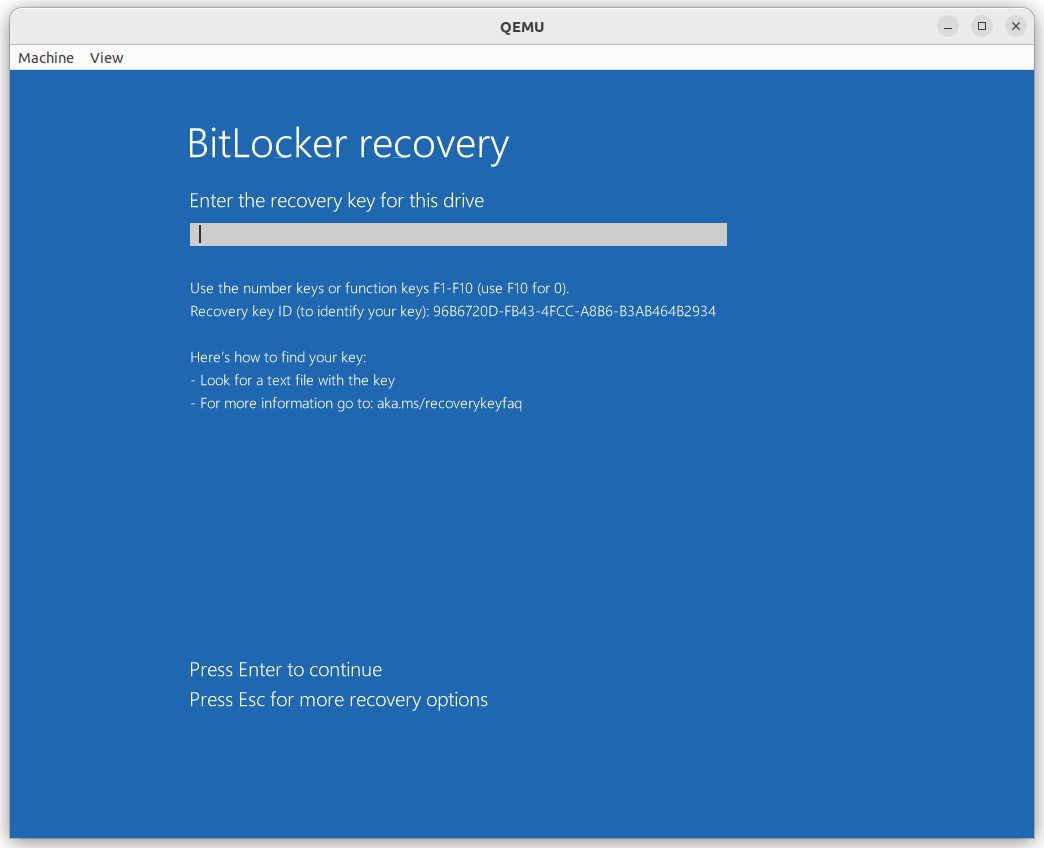
\includegraphics[width=\textwidth]{attacks/bitlocker/01_recovery_prompt.png}

% tpm values different
This happens due to TPM PCR values differing from what was initially used to seal the VMK, leaving the Windows bootloader unable to retrieve an unencrypted VMK from the TPM and as a result unable to decrypt the Windows installation. \TODO{the two different bitlocker volumes}

% bitlocker auto decryption fails
% boot execution differs from executing rootkit
\TODO{which measurements are used for sealing and unsealing}
\TODO{which ones are altered by the rootkit being present}


In theory this is as far as we get, BitLocker in combination of TPM measurements successfully mitigates UEFI attacks by disovering a deviation in the boot flow.
% what is the reaction of the average user
In practice we have to ask ourselves the question how a user reacts to seeing the BitLocker recovery prompt and the consequences to the action the user takes. As an immediate reaction the user has two options: entering the recovery key into the prompt or not entering the recovery key.
% motivation behind user decision
What decision the user makes is dependent on their tech saviness and influenced by a variety of factors such as urgency of booting into Windows, knowing alternatives to what the prompt tells them.
It is reasonable to assume that the average user is willingly entering their recovery key in response to the prompt as the prompt does not suggest any malicious causes or any negative reprocussions in following the instructions. The link mentioned in the prompt also only aids in locating the reocvery key \cite{microsoft-recovery-key-faq}.
\TODO{mention microsofts reasons for the prompt to be triggered}
\TODO{what is the actual alternative}
% does the user trust the system
% why would they not trust the system
% (ask admin for recovery password)
% type in recovery password
% alternative would be to remove drive and insert into safe device

Having the user enter their recovery key does not directly benefit our endevaours as BitLocker does not en/decrypt the hard drive as a whole upon boot but instead performs these respective action when reading or writing a block of data to or from the hard drive.

What we can do is try to record the keystrokes performed by the user while entering their recovery key and use it at some later point to gain control over the hard drive. A program designed to perform this type of attack is called a keylogger.

To implement such a keylogger we have to alter the code execution that happens when the recovery prompt is shown. For this our first step is to find our what execution environment or UEFI stage we are in, is Windows already using separate drivers for keyboard access or still relying on the UEFI environment and its protocols.

% ref to background os loader
% prompt is done by the OS Loader
% ergo still during transient system load phase
% required to use protocol services
% therefor uses uefi services for IO
% such as SimpleTextInputEx Protocol
% go over the two different input protocols
% find out which one is used
The UEFI specification defines two protocols which are used to abstract keyboard input these are the \lstinline{{SimpleTextInputProtocol} and the \lstinline{{SimpleTextInputExProtocol} \cite[12.2, 12.3]{uefi-spec}. To figure out if the recovery prompt uses these to read key strokes we can just add some print statements to the \lstinline{ReadKeyStroke} and \lstinline{ReadKeyStrokeEx} functions of their implementations in the edk2 OVMF package. On the next boot when typing we find that our \lstinline{ReadKeyStrokeEx} print statements from the \lstinline{{SimpleTextInputExProtocol} are triggered.

Now, knowing that the BitLocker recovery prompt is shown by an application running in the UEFI boottime environment, we can leverage this environment to implement our keylogger.

% explain more in depth how protocols are returned to the end user
% one instance per controller/handle
\TODO{how are protocols returned to the end user}
% explain basic back to the caller. This method is called function hooking
% explain how we retain information of the hook in question
% map protocol pointer to hook information
% keylog recovery key
To alter the code execution when performing a key stroke we can just iterate over all instances of the \lstinline{{SimpleTextInputExProtocol} and reassign the \lstinline{ReadKeyStrokeEx} entry of the struct, which is a function pointer. We will save each protocol instances' original function address and instead have it point to an intermediary function. This intermediary calls the original function and performs logging of the key stroke result before relaying the result to the caller. This method is called function hooking and is intransparent to consumer of a protocol.

%  show whole protocol
% WaitForKeyEx event
% wait for event
% query which key it was

\TODO{how is the SimpleTextInputEx Protocol used}

So far we are able to track each keystroke that queried via the \lstinline{ReadKeyStrokeEx} function, which in our testing is only done during the recovery prompt, but may be used by BIOS interactive menu.

\TODO{key input advancment is weird and makes tracking tricky}
F keys
block validity
only divisable by 11
cursor can move out of incomplete or valid blocks
up and down increments or decrements the cursor position

alternatively screen shot
still need hook to find when enter is pressed
explain how screenshotting works
some basic compression
wait for recovery key
send recovery key on enter press

on real hardware
network stack wasn't installed onto handles when boot over ip was disabled
compared loaded dxe drivers between both configurations with efi shell
Realtek Family driver not loaded
load manually
reinstall all handle to controllers to enable network stack regardless

sending key out is only good for physical access attack vector
dislocker linux utility
\cite{dislocker}
mount encrypted drive with decryption mean
read and write access
dual boot in vm
enter recovery key and it works
port to uefi

bitlocker encrypts block-wise

% blk and fs
\TODO{explain block devices}
\TODO{explain file system indepent abstraction better}
uefi protocol stack
\TODO{diagram of block io, disk io, simple filesystem and file protocol interaction (with hindsight of adding dislocker beneath block io)}
\cite[13.3.2 Partition Disocvery]{uefi-spec}
Drivers providing Simple File System Protocol use the Block I/O Protocol to access the underlying media.


hook block io
again hook data mapping

% execute after NTFS driver by doing it in an ExitBootServices hook
It is beneficial for us to write our payload to the Windows installation as close to the end of the UEFI environment as possible, this will maximize the presence of drivers and their offered access to hardware devices. It is also a wise design decision for the attacks following to this one. The call of the function \lstinline{ExitBootServices} marks the point of transitioning from boot time to runtime where the operating system takes over the control of the system, it presents a good opportunity for us to perform the write action of our rootkit.
% was muss man beachten bei exitbootservices hooking
\cite{exitbootservices-hooking}
hook ExitBootServices
enable hook
write payload
import registry key
disable hook

next boot would require to recovery key again
% https://learn.microsoft.com/en-us/windows/security/information-protection/bitlocker/bitlocker-use-bitlocker-drive-encryption-tools-to-manage-bitlocker
update tpm values in payload
caveat pin? look into this

% reference to rootkit definition
persistence when part of root of trust
fresh install / tpm update values
% paper von betreuern
hook Trusted Copmuting Group 2 (TCG2) Protocol
TPM communication
\cite[6.7.3]{tcg-efi-platform-spec}
% \cite[12.7 TPM_Unseal]{tcg-tpm-library-part3-commands}
receive bitlocker vmk key and send to dislocker

% https://labs.withsecure.com/publications/sniff-there-leaks-my-bitlocker-key